\documentclass[11pt]{article}
\usepackage [spanish,active acute] {babel}
\usepackage[utf8]{inputenc}
\usepackage{caption}
\input xy
\xyoption{all}

\usepackage{labels} 
\usepackage{color}
\definecolor{gray97}{gray}{.97}
\definecolor{gray75}{gray}{.75}
\definecolor{gray45}{gray}{.45}

\usepackage{listings}
\lstset{ frame=Ltb,
     framerule=0pt,
     aboveskip=0.5cm,
     framextopmargin=3pt,
     framexbottommargin=3pt,
     framexleftmargin=0.4cm,
     framesep=0pt,
     rulesep=.4pt,
     rulesepcolor=\color{gray97},
     %
     stringstyle=\ttfamily,
     showstringspaces = false,
     basicstyle=\small\ttfamily,
     commentstyle=\color{gray45},
     keywordstyle=\bfseries,
     %
     numbers=left,
     numbersep=15pt,
     numberstyle=\tiny,
     numberfirstline = false,
     breaklines=true,
   }
 
% minimizar fragmentado de listados
\lstnewenvironment{listing}[1][]
   {\lstset{#1}\pagebreak[0]}{\pagebreak[0]}
 
\lstdefinestyle{consola}
   {basicstyle=\scriptsize\bf\ttfamily,
    backgroundcolor=\color{gray75},
   }
 
\lstdefinestyle{C}
   {language=C,
   }
\usepackage{enumerate}

\usepackage{url}

%% Define a new 'leo' style for the package that will use a smaller font.
\makeatletter
\def\url@leostyle{%
  \@ifundefined{selectfont}{\def\UrlFont{\sf}}{\def\UrlFont{\small\ttfamily}}}
\makeatother
%% Now actually use the newly defined style.
\urlstyle{leo}



 \usepackage{algorithm}
 \usepackage{algorithmic}
\floatname{algorithm}{Algoritmo}
\renewcommand{\listalgorithmname}{Lista de algoritmos}
\renewcommand{\algorithmicrequire}{\textbf{Requiere:}}
\renewcommand{\algorithmicensure}{\textbf{Asegura:}}
\renewcommand{\algorithmicend}{\textbf{fin}}
\renewcommand{\algorithmicif}{\textbf{si}}
\renewcommand{\algorithmicthen}{\textbf{entonces}}
\renewcommand{\algorithmicelse}{\textbf{si no}}
\renewcommand{\algorithmicelsif}{\algorithmicelse,\ \algorithmicif}
\renewcommand{\algorithmicendif}{\algorithmicend\ \algorithmicif}
\renewcommand{\algorithmicfor}{\textbf{para}}
\renewcommand{\algorithmicforall}{\textbf{para todo}}
\renewcommand{\algorithmicdo}{\textbf{hacer}}
\renewcommand{\algorithmicendfor}{\algorithmicend\ \algorithmicfor}
\renewcommand{\algorithmicwhile}{\textbf{mientras}}
\renewcommand{\algorithmicendwhile}{\algorithmicend\ \algorithmicwhile}
\renewcommand{\algorithmicloop}{\textbf{repetir}}
\renewcommand{\algorithmicendloop}{\algorithmicend\ \algorithmicloop}
\renewcommand{\algorithmicrepeat}{\textbf{repetir}}
\renewcommand{\algorithmicuntil}{\textbf{hasta que}}
\renewcommand{\algorithmicprint}{\textbf{imprimir}} 
\renewcommand{\algorithmicreturn}{\textbf{devolver}} 
\renewcommand{\algorithmictrue}{\textbf{cierto }} 
\renewcommand{\algorithmicfalse}{\textbf{falso }} 

%\documentclass{acmconf}

\usepackage[paper=a4paper,dvips,top=1.5cm,left=1.5cm,right=1.5cm,
    foot=2cm,bottom=4.5cm]{geometry}



\usepackage{times}
 \usepackage[dvips]{graphicx}
\usepackage[fleqn]{amsmath}
\usepackage{amsfonts}
\usepackage{amssymb}
\usepackage{amsthm}
\usepackage{amsopn}
\usepackage{amstext}
\usepackage{xspace}
% \usepackage{array}
% \usepackage{epsfig}
% \usepackage{easyeqn}

\numberwithin{figure}{section}

\newcommand\CC{\Lang{\mbox{C++}}\xspace}
\newcommand\Lang[1]{\textsc{#1}}
\newcommand{\kw}[1]{\texttt{\textbf{#1}}}
\newcommand{\cd}[1]{\texttt{#1}}

\newcommand\Naturals{\ensuremath{\mathbb{N}}\xspace}
\newcommand\Integers{\ensuremath{\mathbb{Z}}\xspace}
\newcommand\Rationals{\ensuremath{\mathbb{Q}}\xspace}
\newcommand\Reals{\ensuremath{\mathbb{R}}\xspace}
\newcommand\Complex{\ensuremath{\mathbb{C}}\xspace}

\newcommand\norm[1]{\ensuremath{\lVert#1\rVert}}
\newcommand\abs[1]{\ensuremath{\lvert#1\rvert}}
\newcommand\ceil[1]{\ensuremath{\lceil#1\rceil}}
\newcommand\floor[1]{\ensuremath{\lfloor#1\rfloor}}
\newcommand\set[1]{\ensuremath{\{#1\}}}
\newcommand\interval[1]{\ensuremath{[#1]}}
\newcommand\angular[1]{\ensuremath{\langle#1\rangle}}

\newcommand\Norm[1]{\ensuremath{\left\lVert#1\right\rVert}}
\newcommand\Abs[1]{\ensuremath{\left\lvert#1\right\rvert}}
\newcommand\Ceil[1]{\ensuremath{\left\lceil#1\right\rceil}}
\newcommand\Floor[1]{\ensuremath{\left\lfloor#1\right\rfloor}}
\newcommand\Set[1]{\ensuremath{\left\{#1\right\}}}
\newcommand\Interval[1]{\ensuremath{\left[#1\right]}}
\newcommand\Angular[1]{\ensuremath{\left\langle#1\right\rangle}}

\newtheorem{theorem}{Theorem}[section]
\newtheorem{definition}[theorem]{Definition}
\newtheorem{lemma}[theorem]{Lemma}
\newtheorem{corollary}[theorem]{Corollary}
\newtheorem{fact}[theorem]{Fact}
\newtheorem{example}[theorem]{Example}

\newcommand\Cls[1]{\textsf{#1}}
\newcommand\Fig[1]{Figura~\ref{Figura:#1}}
\newcommand\Lin[1]{Línea~\ref{lin:#1}}
\newcommand\Alg[1]{Algoritmo~\ref{alg:#1}}
\newcommand\lin[1]{(\ref{lin:#1})}

\newenvironment{excerpt}{\begin{quote}\begin{minipage}\textwidth}{\end{minipage}\end{quote}}

\setcounter{topnumber}{0}
\setcounter{bottomnumber}{0}
\setcounter{totalnumber}{20}
\renewcommand{\textfraction}{0.01}
\pagestyle{plain}

\usepackage{caratula}
 \usepackage{fancyhdr}
 \usepackage{graphicx}

 \pagestyle{fancy}
 \lhead{{\footnotesize \texttt{Grupo POPA}}} %aca ira el numero de grupo despues
 \chead{}
 \rhead{{\footnotesize \texttt{Cerrutti - Huel - Mita}}}
 \lfoot{}
 \cfoot{}
 \cfoot{\thepage\ /~\pageref{'lastPage'}}
 \rfoot{}

\headsep = 30pt
\footskip = 20pt

\makeatletter
\newenvironment{breakalgo}[2][alg:\thealgorithm]{%
  \def\@fs@cfont{\bfseries}%
  \let\@fs@capt\relax%
  \par\noindent%
  \medskip%
  \rule{\linewidth}{.8pt}%
  \vspace{-3pt}%
  \captionof{algorithm}{#2}\label{#1}%
  \vspace{-1.7\baselineskip}%
  \noindent\rule{\linewidth}{.4pt}%
  \vspace{-1.3\baselineskip}%
}
{
	\vspace{-.75\baselineskip}
	\rule{\linewidth}{.4pt}serverPutete

	\medskip
}
\makeatother
\begin{document}



\materia{Algoritmos y Estructuras de Datos III}

\titulo{Trabajo Practico 3}

\grupo{Grupo 15}

\integrante{Mariano Javier Cerrutti}{525/07}{vscorza@gmail.com}

\integrante{Federico xxx Huel}{xxx/07}{federico.huel@gmail.com}

\integrante{Rogelio xxx Mita}{xxx/07}{rogeliomita@gmail.com}

\maketitle

\tableofcontents

\newpage
\section{Presentación}
El propósito de este trabajo es presentar una solución al problema de
\emph{detección de bordes en una imagen digital} a través de un operador definido por una matriz de convolución.


Acá hay un poco de sarasa matemática:\\
\begin{center}
\begin{minipage}{5in}
Sea $p$ pixel, $|p|=4$ y una imagen $I = {p_{i,j} : i \in ancho, j \in alto}$ se aplicará el operador sobel en x
\[ \left( \begin{array}{ccc}
-1 & 0 & 1 \\
-2 & 0 & 1 \\
-1 & 0 & 1 \end{array} \right)\]

\end{minipage}
\end{center}



\newpage
\section{Propuesta}
Acá mandamos una propuesta? No se como armamos en general el reporte.\\
Un grafo por si hay que meter alguno después

\begin{figure}[H]
	\centerline{
		\xymatrix{ & Luisa(90) \ar@{<->}@/_2ex/[dl] \ar@{<->}@/^2ex/[dr]&\\
		Analia(50) \ar@{<->}@/^2ex/[drr] & & Florenzia(20) \ar@{<->}@/_2ex/[dll] \\
		Romina(30) \ar@{<->}@/_2ex/[rr] & & Carla(60)\\
		& Betty(5)&}
	}
	\caption{El grafo de intimidades.}
	\label{fig:grafoIntimidades}
\end{figure}

\newpage
\section{Algoritmo}
\subsection{Introducción}
Acá metemos la descripción del algoritmo.
\subsection{Desarrollo}
Explicamos el algo.
\subsection{Pseudoc\'odigo}
Acá metemos el pseudo.

Esto será recorrido así, sarasa de pseudocódigo:
\begin{breakalgo}{SobelEnX}
 \begin{algorithmic}[1]
\STATE I $\leftarrow {p_{i,j} : i \in ancho, j \in alto}$
\FOR{$i \in ancho$}
\FOR{$j \in alto$}
\STATE $p_{i,j} \leftarrow -p_{i-1,j-1} - 2 * p_{i-1,j} - p_{i-1,j+1} +p_{i+1,j-1} + 2 * p_{i+1,j} + p_{i+1,j+1}$\label{lin:linea_asignapixel}
\ENDFOR
\ENDFOR
 \end{algorithmic}
\end{breakalgo}

\subsection{Detalles de implementación}
Acá puede ir todo o parte del asm.

\begin{lstlisting}[language={[x86masm]Assembler}]
 asmSobel:
	doEnter 1
	
	cmp dword XORDER, 0
	je	ySobel

	xSobel:
	;==========================
	; SOBEL XORDER
	;==========================
	mov eax, HEIGHT
	mov dword T_HEIGHT, eax

	mov	edx,	SRC
	mov	edi,	[edx + WIDTH_STEP]
	
	mov	ecx,	SRC		;ecx registro para el pixel de origen
	mov	ecx,	[ecx + IMAGE_DATA]

	mov	esi,	DST		;esi registro para el pixel de destino
	mov	esi,	[esi + IMAGE_DATA]

	add	esi,	edi		;salteo la primera linea
	inc	esi			;salteo la primer columna

	cicloY:
	 mov edx, edi
	  sub	edx,	2		;le resto los pixeles laterales

	  add	ecx,	2		;sumo dos para llevar al primero de la linea siguiente
	  add	esi,	2

	  cicloX:
	      mov	eax,	[ecx]	;cargo cuatro pixeles en eax
	      and	eax,	0x00FF00FF	;paso a dos words empaquetadas
	      ;shr	eax,8	;desplazo ocho bits a derecha para permitir operaciones en 8 bits
	      mov	ebx,	[ecx + edi]	;sumo dos veces la segunda linea
	      and	ebx,	0x00FF00FF	;paso a dos words empaquetadas
	      shl	ebx,1	;desplazo siete bits a derecha para permitir operaciones en 8 bits
	      add	eax,	ebx
	      mov	ebx,	[ecx + edi * 2]	;sumo la tercera linea
	      and	ebx,	0x00FF00FF	;paso a dos words empaquetadas
	      ;shr	ebx,	8	;desplazo ocho bits a derecha para permitir operaciones en 8 bits
	      add	eax,	ebx
	      mov	ebx,	eax
	      shr	eax,	16	;muevo eax a la parte izquierda de la matriz
	      sub	ax,	bx	;se la resto al pixel destino
	      cmp	ax,	0x00FF
	      jg	sobresaturo
	      cmp	ax,	0x0000
	      jl	subsaturo
	      volver:

	      add	[esi],	al	;mando el pixel
	      inc	ecx
	      inc	esi
	      dec edx
	      jnz cicloX
	  dec	dword T_HEIGHT
	  jnz	cicloY
	jmp pintaBordes

	ySobel:

	cmp dword YORDER, 0
	je	pintaBordes
\end{lstlisting}


\subsection{C\'alculo de complejidad}
Hacemos cálculo de complejidad?\\
Para referenciar una línea es así:

\textbf{\lin{linea_asignapixel}} O(1) $\rightarrow$ ya que es una gilada.\\

\subsection{Demostración}
Demostramos que el algoritmo realmente hace lo que nos piden?





\subsection{Análisis}
Acá tendríamos que analizar la respuesta de nuestro algoritmo respecto del de opencv.\\

Un ejemplo de tabla:
\begin{center}
\begin{tabular}{|c c | c c c c | c |}
\hline
$n$ 	& densidad &	Orden HC & Iters. GRASP & Iters. s/mejora & Iters. HBL &
Dist. al exacto\\
\hline
10 & 100 & 10 & 10 & 3 & 1 & 0\\
10 & 100 & 10 & 10 & 3 & 1 & 0\\
\ldots& \ldots & \ldots & \ldots & \ldots & \ldots & \ldots\\
50 & 75 & 10 & 10 & 3 & 1 & 0\\
50 & 75 & 10 & 10 & 3 & 1 & 0\\
50 & 75 & 10 & 10 & 3 & 1 & 0\\
\hline
\end{tabular}
\end{center}

Un ejemplo de gráfico:\\
\begin{center}
\begin{figure}[H]
	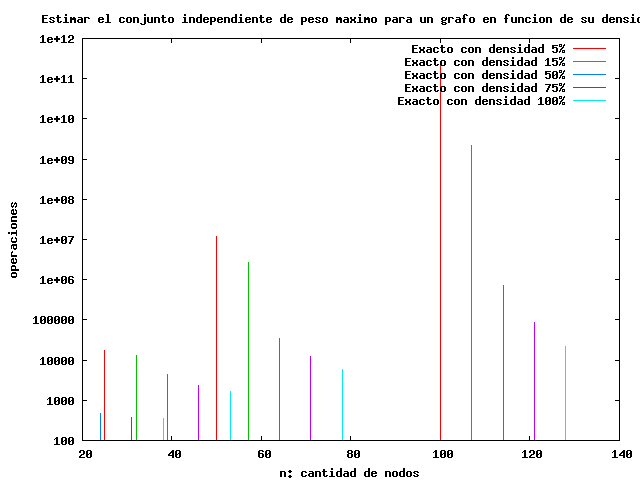
\includegraphics[scale=.7,natwidth=640pt,
	natheight=480pt]{img/tiempos.png} \caption{Tiempos de ejecución del algoritmo SARASA}
	\label{fig:mwispGraspSinMejoraOps}
\end{figure}
\end{center}
\newpage

\section{Conclusiones}
Acá metemos las conclusiones del trabajo?
\label{'lastPage'}
\end{document}